\documentclass[10pt]{beamer}

\mode<presentation>
{
  \usetheme[height=1.25cm]{Madrid}
  \setbeamertemplate{navigation symbols}{}
  \setbeamercolor{alerted text}{fg=illini}
}
\graphicspath{{./}{figs/}{/Users/hic/Dropbox/To-process/slides/pics/}{/Users/hic/Dropbox/To-process/slides/pics/feat-det/}{/Users/hic/Dropbox/To-process/slides/3630-08/}{/Users/hic/Dropbox/To-process/slides/8803-09/}{/Users/hic/Dropbox/To-process/slides/8803-12/}{/Users/hic/Dropbox/To-process/slides/8803-08/}}

\usebackgroundtemplate{
\includegraphics[width=\paperwidth,height=\paperheight]{uc-background}}

\usepackage[english]{babel}
\usepackage{epsfig,subfigure,bm}
\usepackage{multimedia}
\usepackage{psfrag}
\usepackage{animate}

% \usefonttheme{metropolis} % default family is serif
%%%%%% Begin of my macros and options

\setbeamertemplate{section in toc shaded}[default][55]
\setbeamertemplate{subsection in toc shaded}[default][55]
\setbeamercolor{block title}{fg=white,bg=illini}
\setbeamercolor{block body}{fg=black,bg=mygrey}

\setbeamercolor{emphprimary}{fg=CBlue}
\setbeamercolor{emphsecondary}{fg=illini}
\setbeamercolor{emphtertiary}{fg=mygreen}
\definecolor{darkForestGreen}{rgb}{.1,1,.1}
\definecolor{veryLightGray}{rgb}{.9,.9,.9}
\definecolor{greenApple}{rgb}{.3,.9,.3}

\setbeamercolor{title}{bg=CBlue}

\usepackage{amsmath,amssymb,amsxtra,amsthm}
\usepackage{algorithm,algorithmic}
\usepackage{natbib}
\usepackage{bibentry}
\usepackage{xspace}
\usepackage{changepage}

\definecolor{myblue}{rgb}{.2,.2,.7}
\definecolor{myred}{rgb}{.7,.2,.2}
\definecolor{mygreen}{rgb}{.2,.7,.2}
\definecolor{mygrey}{rgb}{0.9,0.9,0.9}
\definecolor{CBlue}{cmyk}{1,0.25,0,0}
\definecolor{illini}{rgb}{0.98,0.4,0.05}
\definecolor{black}{cmyk}{0,0,0,1}

\newcommand{\myemph}[1]{{\usebeamercolor[fg]{emphprimary}
    \textbf{#1}}}
\newcommand{\myemphalt}[1]{{\usebeamercolor[fg]{emphsecondary}
    \textbf{#1}}}


\title[Math for Robotics] % (optional, use only with long paper titles)
{CSE276C - Markov Chains}

\author[H.~I. Christensen] % (optional, use only with lots of authors)
{Henrik I.~Christensen}
% - Give the names in the same order as the appear in the paper.  -
% Use the \inst{?} command only if the authors have different
% affiliation.

\AtBeginSection[]
{
   \begin{frame}
       \frametitle{Outline}
       \tableofcontents[currentsection]
   \end{frame}
}

\institute[UCSD] % (optional, but mostly needed)
{
  \begin{minipage}[c]{.2\textwidth}
    
\includegraphics[width=.65\linewidth]{ucsealnew}%
  \end{minipage}%
  \begin{minipage}[c]{.6\textwidth}
    \small
%%    \begin{center}
      Computer Science and Engineering\\
      University of California, San Diego\\
%%    \end{center}

  \end{minipage}
%%  \vspace*{1ex}
}
%% - Use the \inst command only if there are several affiliations.
%% - Keep it simple, no one is interested in your street address.

\bigskip

\date[Nov 2021]% (optional, should be abbreviation of conference name)
{\small%
  November 2021}

\begin{document}

\nobibliography{/Users/hic/Dropbox/bibliography/bib-file.bib}
\bibliographystyle{plain}

\begin{frame}[plain]
  \titlepage
\end{frame}


\begin{frame}
  \frametitle{Introduction}
  \begin{itemize}
  \item How do we model temporal ``discrete'' processes with
    associated uncertainty?
  \item Lots of examples in robotics
    \begin{itemize}
    \item Executing a plan
    \item Modeling traffic
    \item Receiving packages for logistics
    \end{itemize}
  \item Basic coverage of the underlying theory
  \end{itemize}
\end{frame}

\begin{frame}
  \frametitle{Independent Trials}
  \begin{itemize}
  \item A set of possible outcomes $X_1, X_2, \ldots$ is given
  \item Each outcome has an associated probability $p_k$
  \item The probability of a samples sequence is given by
    \[
      P \{ (X_{j0}, X_{j1}, \ldots, X_{jk}) \} = p_{j0} p_{j1} \cdots p_{jk}
    \]
  \end{itemize}
\end{frame}

\begin{frame}
  \frametitle{Markov Chains -- Introduction}
  \begin{itemize}
  \item The outcome of any trial dependent on the outcode of the
    directly precedings trial only
  \item \myemph{Conditional Probability $p_{jk}$}: given $X_j$ has
    occured at some trial the probability of $X_k$ at the next trial
  \item $a_k$ is the probability of $X_k$ at the initial trial
  \item I.e.:
    \[
      \begin{array}{rcl}
        P\{ ( X_j, X_k) \} &=& a_k p_{jk}\\
        P\{ ( X_j, X_k, X_l) \} &=& a_j p_{jk} p_{kl}\\
        P \{ (X_{j0}, X_{j1}, \ldots, X_{jk}) \} &=& a_{j0} p_{j1} \cdots p_{jk}\\
      \end{array}
    \]
  \end{itemize}
\end{frame}

\begin{frame}
  \frametitle{Example -- Random Walk}
  \begin{itemize}
  \item How would you model a random walk? \pause
  \item Events: $\{ \ldots, -3, -2, -1, 0, 1, 2, 3, \ldots \}$
  \item $p_{ij} = 0$ if $|j-k| > 1$
  \item $p_{ij} = \frac{1}{2} \mbox{ for } |i-j| = 1$
  \end{itemize}
  \centerline{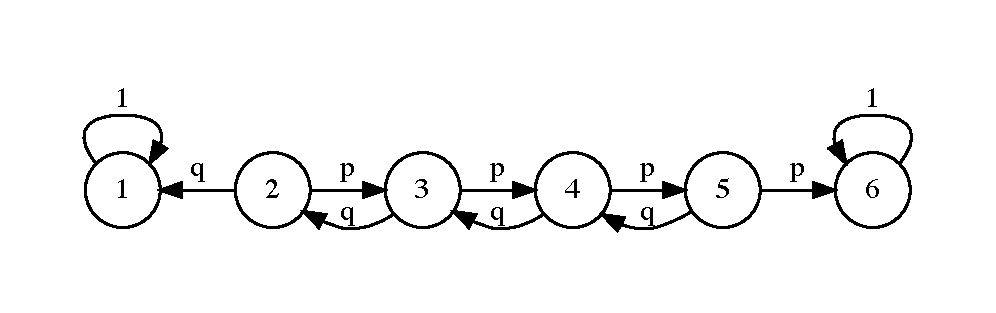
\includegraphics[height=2.5cm]{basic-mc}}
\end{frame}

\begin{frame}
  \frametitle{Formalizing things}
  \begin{itemize}
  \item The chain is in a \myemph{state} $X_t$ at time t.
  \item The \myemph{state space} of a chain is the value X can take
    on, i.e., $S = \{ 1, 2, 3, 4, 5, 6\}$. Let the size of S be N
    (possibly infinite)
  \item A \myemph{trajectory} of a chain is the set of values of X over time, say
    $X_0, X_1, X_2, \ldots$ The trajectory is the ``path'' through a chain.
  \item The \myemph{Markov Property} implies that the future
    state/trajectory only depends upon the current state, i.e.:
    \[
      P(X_{t+1} = s | X_t = s_t, X_{t-1} = s_{t-1}, \ldots, X_0 = s_0) = P(X_{t+1} = s | X_t = s_t)
    \]
  \item A sequence of discrete events random variables can be
    considered a Markov chain if it satisfies the above property
  \end{itemize}
\end{frame}

\begin{frame}
  \frametitle{Transition matrix}
  \begin{itemize}
  \item We have already seen multiple \myemph{transition diagrams} as shown below for San Diego weather
    \centerline{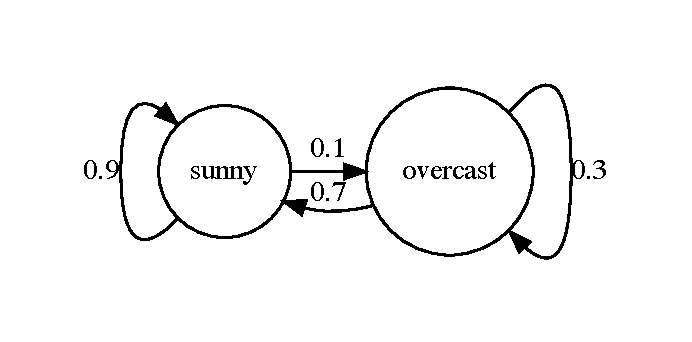
\includegraphics[height=3cm]{sd-weather}}
  \item We can capture the same information in a \myemph{transition
      matrix} -- $(S \times S)$ that details the transitions between states
    \[
      \left(
        \begin{array}{cc}
          0.9 & 0.1\\
          0.7 & 0.3\\
        \end{array}
      \right)
    \]
  \item The transition matrix is one of the most important tools for
    analyzing Markov Chains
  \end{itemize}
\end{frame}

\begin{frame}
  \frametitle{Transition Matrix}
  \begin{itemize}
  \item The transition matrix is frequently denoted $P = (p_{ij})$
  \item In the transition matrix P:
    \begin{itemize}
    \item the ROW represent NOW or FROM ($X_t$)
    \item the COLUMNS present NEXT or TO ($X_{t+1}$)
    \item an entry (i,j) is the CONDITIONAL probability that NEXT (j) is happening given that NOW (i). Expressed as
      \[
        p_{ij} = P(X_{t+1} | X_t)
      \]
    \item Square ($N \times N$) matrix
    \item Rows sum to 1
    \item Columns do not sum to 1
    \end{itemize}
  \end{itemize}
\end{frame}

\begin{frame}
  \frametitle{Initial state}
  \begin{itemize}
  \item The Markov chair also has an initial state $X_0$ which is a
    distribution over possible start states
  \item The initial distirbution is represented by the earlier mentioned $a_i$
  \end{itemize}
\end{frame}


\begin{frame}
  \frametitle{Markov chains}
  \begin{center}
    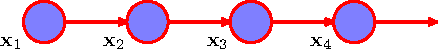
\includegraphics[width=8cm]{prml-Figure13-3}\\[2cm]

    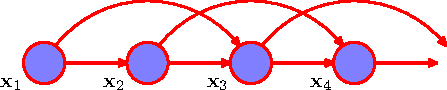
\includegraphics[width=8.4cm]{prml-Figure13-4}
  \end{center}
\end{frame}


\begin{frame}
  \frametitle{Hidden Markov Model}
  \begin{center}
    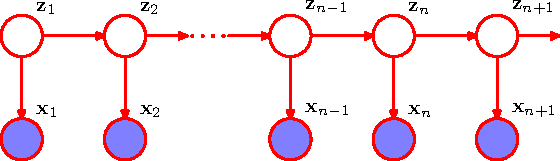
\includegraphics[width=9cm]{prml-Figure13-5}
  \end{center}
\end{frame}



\begin{frame}
  \frametitle{Modelling of HMM's}
  \begin{itemize}
  \item We can model the transition probabilities as a table
    \[
    A_{jk} = p(z_{nk} = 1 | z_{n-1,j} = 1)
    \]
  \item The conditionals are then (with a 1-out-of-K coding)
    \[
    p(z_n|z_{n-1},A) = \prod_{k=1}^K\prod_{j=1}^K A_{jk}^{z_{n-1,j} z_{nk}}
    \]
  \item The per element probability is expressed by $\pi_k =
    p(z_{1k}=1)$
    \[
    p(z_1 | \pi) = \prod_{k=1}^K \pi_k^{z_{1k}}
    \] with $\sum_k \pi_k = 1$
  \end{itemize}
\end{frame}

\begin{frame}
  \frametitle{Illustration of HMM}
  \begin{center}
    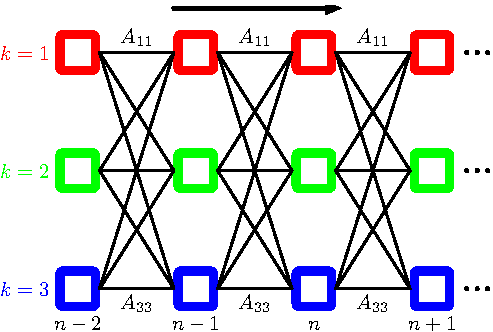
\includegraphics[width=7cm]{prml-Figure13-7}
  \end{center}
\end{frame}


\begin{frame}
  \frametitle{Maximum likelihood for the HMM}
  \begin{itemize}
  \item If we observe a set of data $X=\{ x_1, \ldots, x_N\}$ we can
    estimate the parameters using ML
    \[ p(X|\theta)=\prod_Z p(X, Z| \theta) \]
  \item I.e. summation of paths through lattice
  \item We can use EM as a strategy to find a solution
  \item E-Step: Estimation of $p(Z|X, \theta^{old})$
  \item M-Step: Maximize over $\theta$ to optimize
  \end{itemize}
\end{frame}

\begin{frame}
  \frametitle{ML solution to HMM}
  \begin{itemize}
  \item Define
    \begin{eqnarray*}
      Q(\theta,\theta^{old})&=&\sum_Z p(Z|X, \theta^{old}) \ln p(X,Z|\theta)\\
      \gamma(z_n)&=& p(z_n|X, \theta^{old})\\
      \gamma(z_{nk}) &=& E[z_{nk}] = \sum_z \gamma(z) z_{nk}\\
      \xi(z_{n-1}, z_n) &=& p(z_{n-1}, z_n| X, \theta^{old})\\
      \xi(z_{n-1,j}, z_{nk}) &=& \sum_z \gamma(z) z_{n-1,j} z_{nk}
    \end{eqnarray*}
  \end{itemize}
\end{frame}

\begin{frame}
  \frametitle{ML solution to HMM}
  \begin{itemize}
  \item The quantities can be computed
    \begin{eqnarray*}
      \pi_k &=& \frac{\gamma(z_{1k})}{\sum_{j=1}^K \gamma(z_{1j})}\\
      A_{jk} &=& \frac{\sum_{n=2}^N \xi(z_{n-1,j}, z_{nk})}{
        \sum_{l=1}^K \sum_{n=2}^N \xi(z_{n-1,j}, z_{nl})}
    \end{eqnarray*}
  \item Assume $p(x|\phi_k) = N(x|\mu_k, \Sigma_k)$ so that
    \begin{eqnarray*}
      \mu_k &=& \frac{\sum_n \gamma(z_{nk}) x_n}{\sum_n
        \gamma(z_{nk})}\\
      \Sigma_k &=& \frac{\sum_n \gamma(z_{nk}) (x_n - \mu_k)(x_n - \mu_k)^T}{
        \sum_n \gamma(z_{nk})}
    \end{eqnarray*}
  \item How do we efficiently compute $\gamma(z_{nk})$?
  \end{itemize}
\end{frame}

\begin{frame}
  \frametitle{Forward-Backward / Baum-Welch}
  \begin{itemize}
  \item How can we efficiently compute $\gamma()$ and $\xi(.,.)$?
  \item Remember the HMM is a tree model
  \item Using message passing we can compute the model efficiently
    (remember earlier discussion?)
  \item We have two parts to the message passing forward and backward
    for any component
  \item We have
    \[
    \gamma(z_n) = p(z_n|X) = \frac{P(X|z_n) p(z_n)}{p(X)}
    \]
  \item From earlier we have
    \[
    \gamma(z_n) = \frac{\alpha(z_n)\beta(z_n)}{p(X)}
    \]
  \end{itemize}
\end{frame}

\begin{frame}
  \frametitle{Forward-Backward}
  \begin{itemize}
  \item We can then compute
    \begin{eqnarray*}
      \alpha(z_n) &=& p(x_n|z_n)\sum_{z_{n-1}} \alpha(z_{n-1}) p(z_n|z_{n-1})\\
      \beta(z_n) &=& \sum_{z_{n+1}} \beta(z_{n+1}) p(x_{n+1}|z_{n+1})
      p(z_{n+1}|z_n)\\
      p(X) &=& \sum_{z_n} \alpha(z_n)\beta(z_n)\\
      \xi(z_{n-1}, z_n) &=& \frac{\alpha(z_{n-1})p(x_n|z_n)p(z_n|z_{n-1})\beta(z_n)}{p(X)}
    \end{eqnarray*}
  \end{itemize}
\end{frame}

\begin{frame}
  \frametitle{Sum-product algorithms for the HMM}
  \begin{itemize}
  \item Given the HMM is a tree structure
  \item Use of sum-product rule to compute marginals
  \item We can derive a simple factor graph for the tree
    \begin{center}
      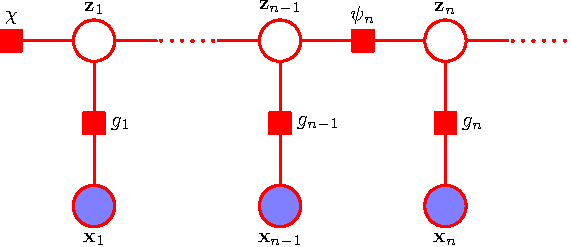
\includegraphics[height=3cm]{prml-Figure13-14}
    \end{center}
  \end{itemize}
\end{frame}

\begin{frame}
  \frametitle{Sum-product algorithms for the HMM}
  \begin{itemize}
  \item We can then compute the factors
    \begin{eqnarray*}
      h(z_1) &=& p(z_1) p(x_1 | z_1)\\
      f_n(z_{n-1}, z_n) &=& p(z_n|z_{n-1}) p(x_n|z_n)\\
    \end{eqnarray*}
  \item The update factors $\mu_{f_n \rightarrow z_n}(z_n)$ can be
    used to derive message passive with $\alpha(.)$ and $\beta(.)$
  \end{itemize}
\end{frame}

\begin{frame}
  \frametitle{Viterbi Algorithm}
  \begin{itemize}
  \item Using the message passing framework it is possible to
    determine the most likely solution (ie best recognition)
  \item Intuitively
  \item Keep only track of the most likely / probably path through the
    graph
  \item At any time there are only K possible paths to maintain
  \item Basically a greedy evaluation of the best solution
  \end{itemize}
\end{frame}

\begin{frame}
  \frametitle{Small example of gesture tracking}
  \begin{itemize}
  \item Tracking of hands using an HMM to interpret track
  \item Pre-process images to generate tracks
    \begin{itemize}
    \item Color segmentation
    \item Track regions using Kalman Filter
    \item Interpret tracks using HMM
    \end{itemize}
  \end{itemize}
\end{frame}

\begin{frame}
  \frametitle{Pre-process architecture}
  \begin{center}
    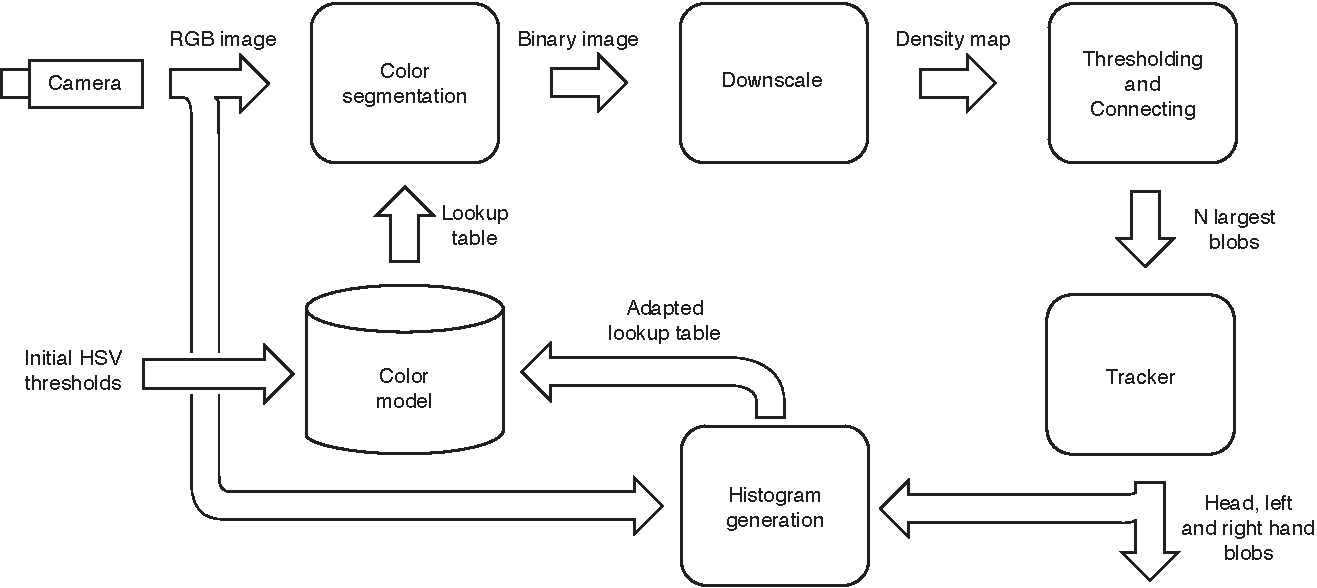
\includegraphics[width=9cm]{gesture-pre-process}
  \end{center}
\end{frame}

\begin{frame}
  \frametitle{Basic idea}
  \begin{center}
    \begin{tabular}[c]{cc}
      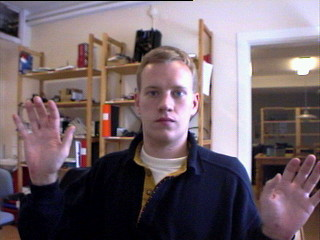
\includegraphics[width=3.5cm]{fredrik-original} &
      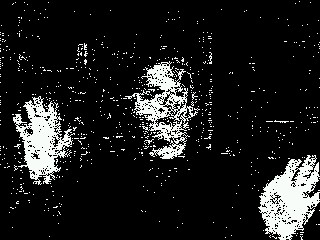
\includegraphics[width=3.5cm]{skin-pixels} \\
      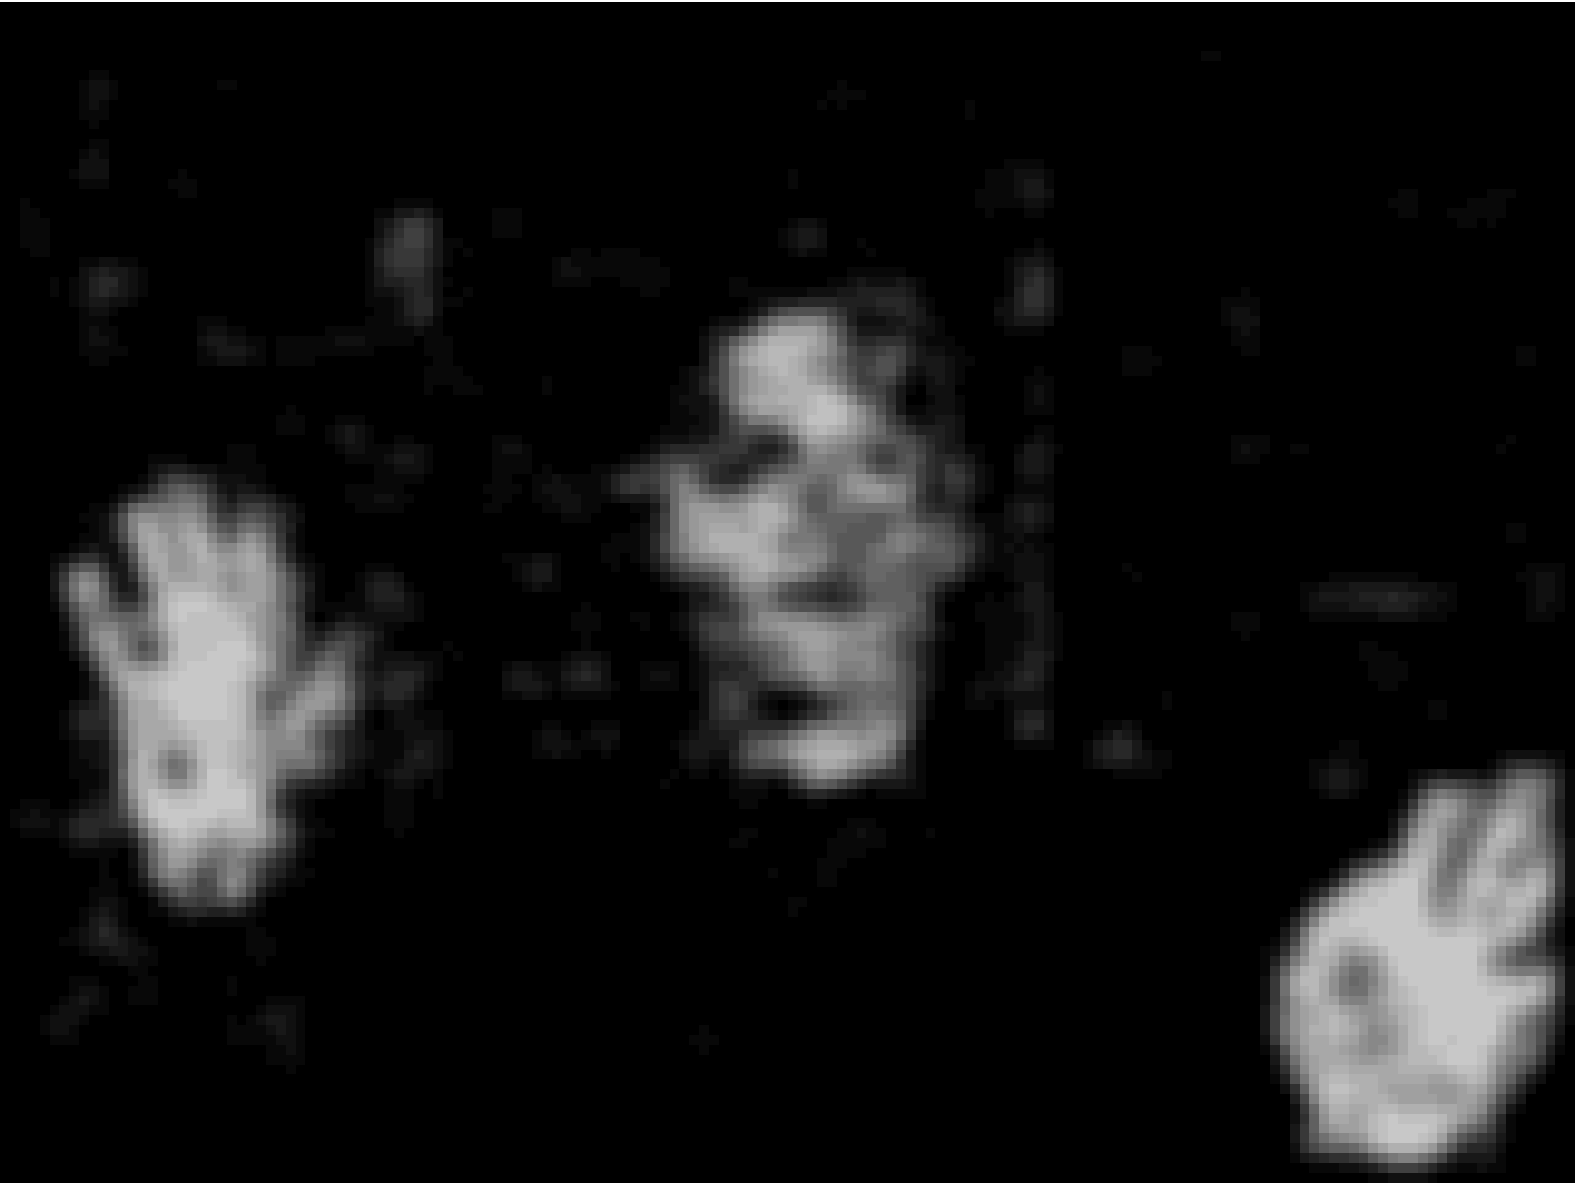
\includegraphics[width=3.5cm]{skin-density} &
      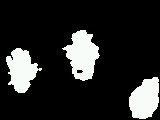
\includegraphics[width=3.5cm]{skin-components}
    \end{tabular}
  \end{center}
\end{frame}

\begin{frame}
  \frametitle{Tracking}
  \begin{center}
    \begin{tabular}[c]{cc}
      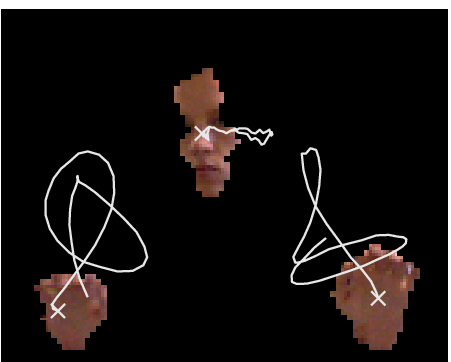
\includegraphics[width=4cm]{gesture-tracking} &
      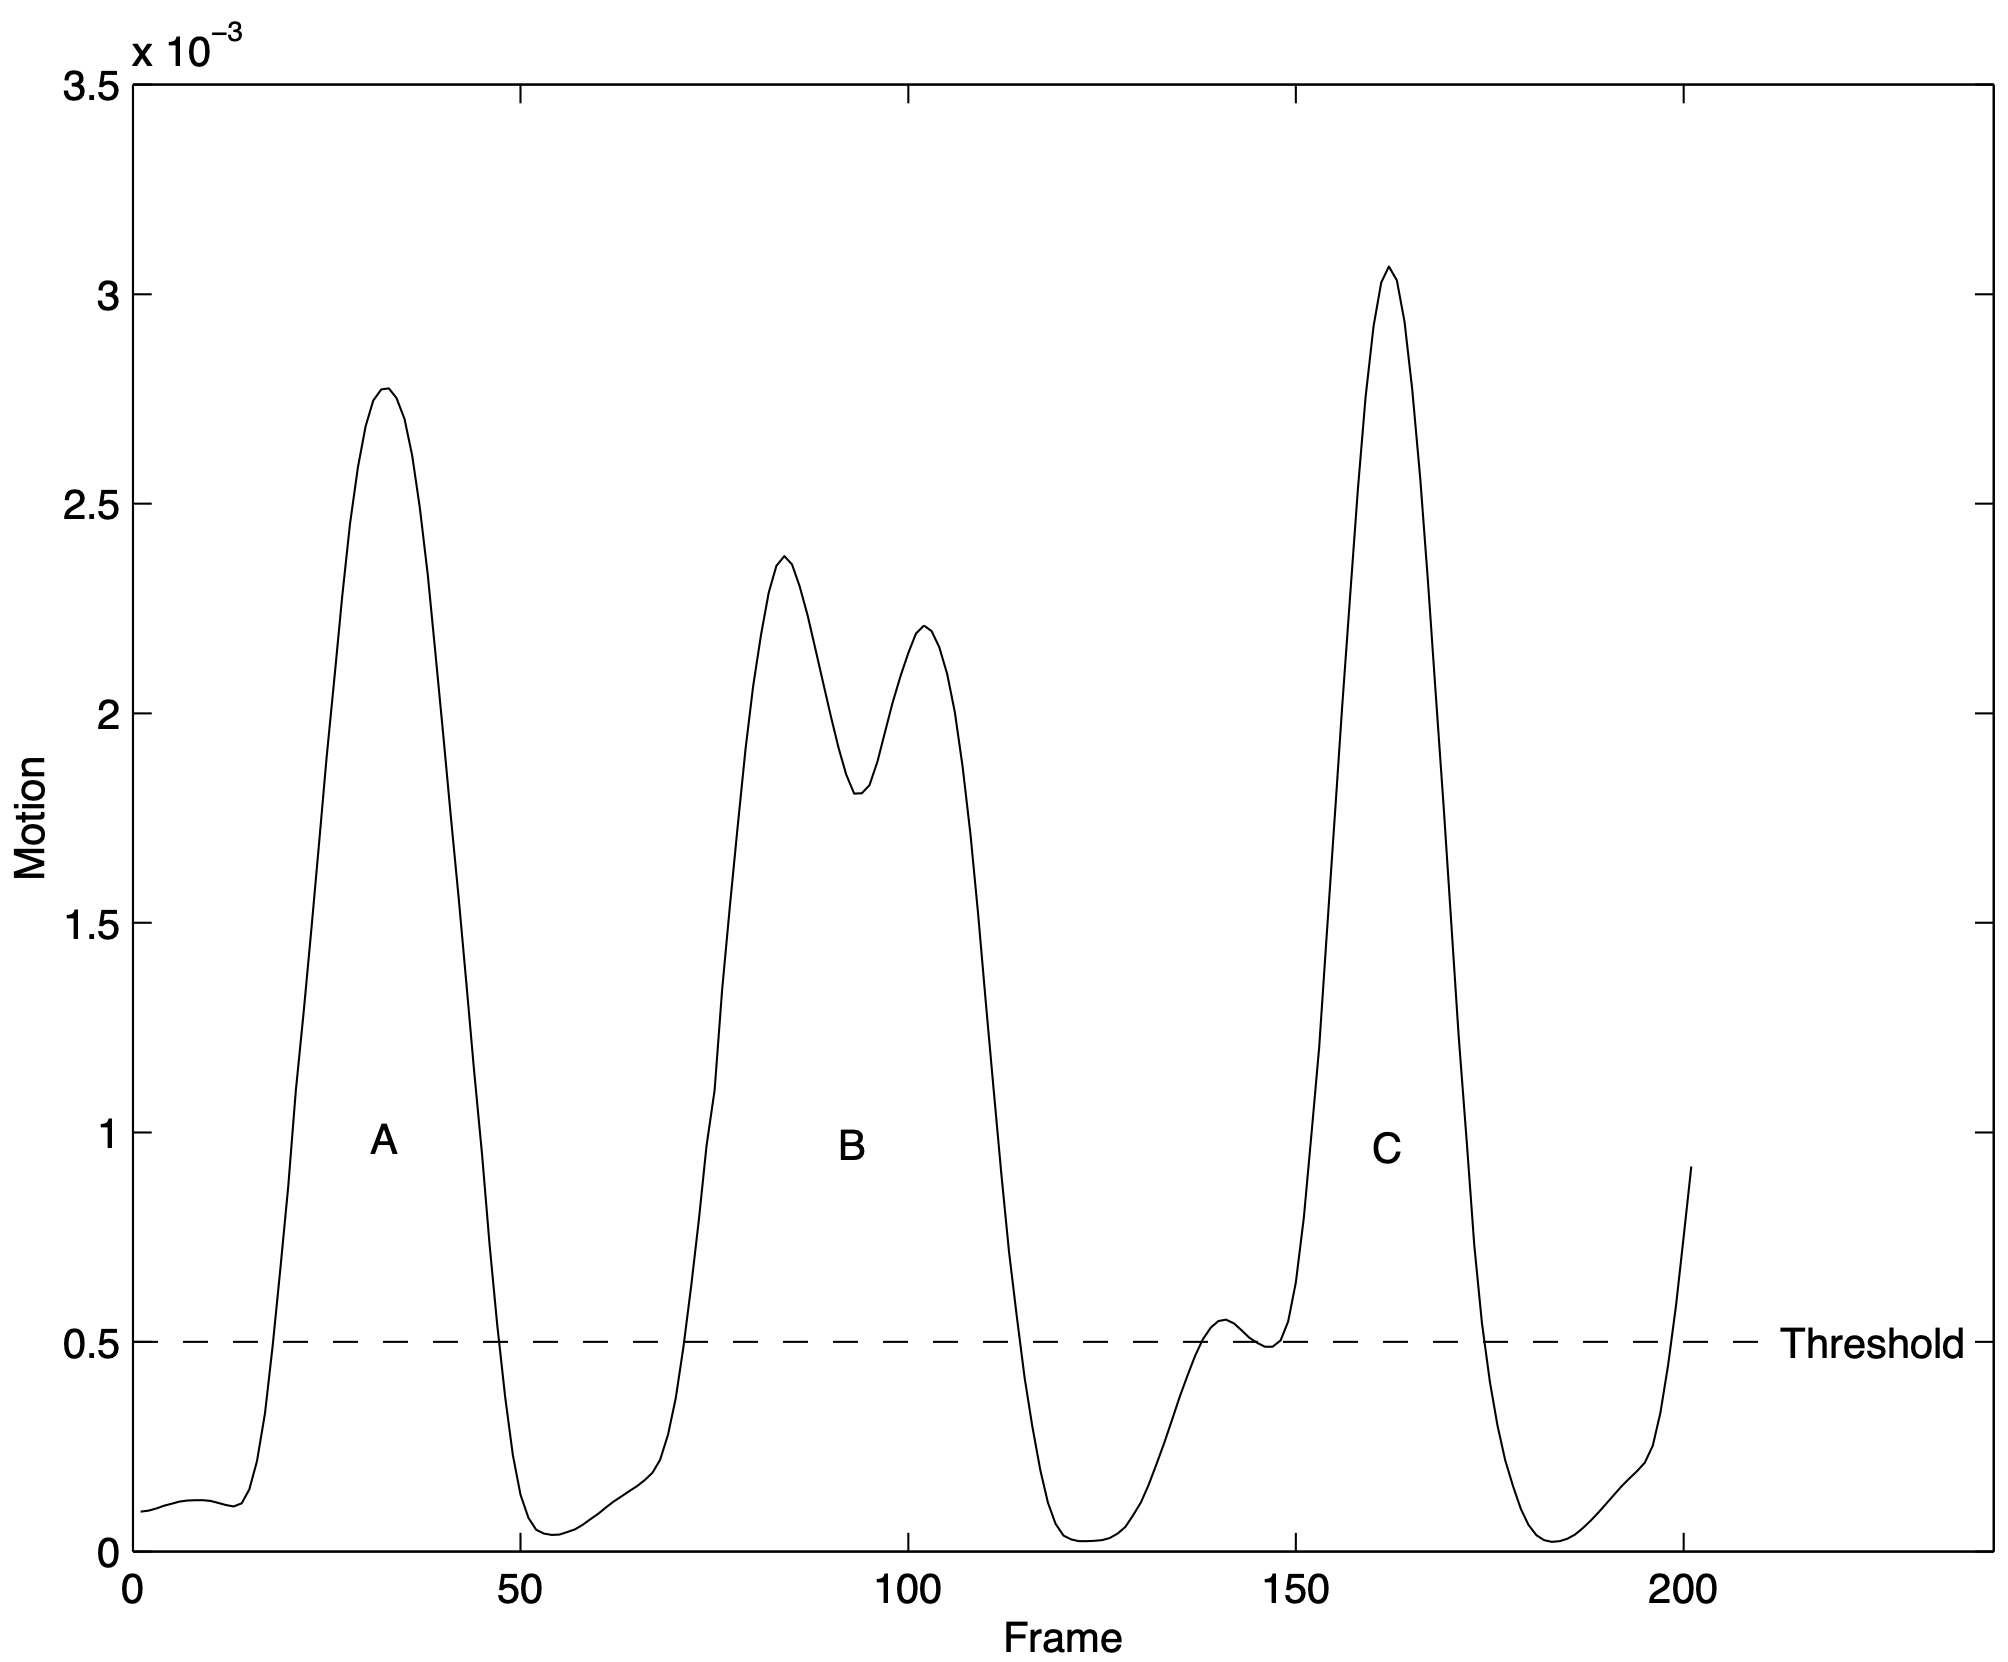
\includegraphics[width=4cm]{gesture-motion}
    \end{tabular}
  \end{center}
\end{frame}

\begin{frame}
  \frametitle{Motion Patterns}
  \begin{center}
    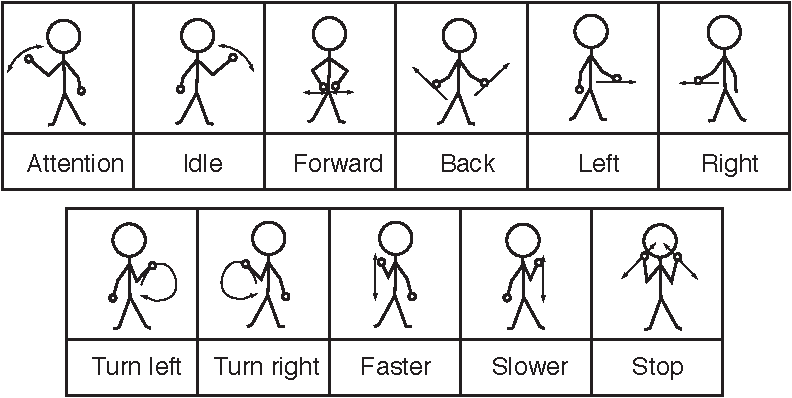
\includegraphics[width=9cm]{airport-gestures}
  \end{center}
\end{frame}

\begin{frame}
  \frametitle{Evaluation}
  \begin{itemize}
  \item Acquired 2230 image sequences
  \item Covering 5 people in a normal living room
  \item 1115 used for training
  \item 1115 sequences were used for evaluation
  \item Capture of position and velocity data
    \begin{tabular}[c]{|c|c|c|c|}
      \hline
      Rec Rates & Position & Velocity & Combined \\ \hline\hline
      Result [\%]& 96.6 & 88.7 & 99.5 \\ \hline
    \end{tabular}
  \end{itemize}
\end{frame}

\begin{frame}
  \frametitle{Example Timing}
  \begin{center}
    \begin{tabular}[c]{|l|c|} \hline
      Phase & Time/frame[ms]\\ \hline\hline
      Image Transfer & 4.3\\
      Segmentation & 0.6\\
      Density Est & 2.1\\
      Connect Comp & 2.1 \\
      Kalman Filter & 0.3 \\
      HMM & 21.0 \\ \hline
      Total & 30.4 \\\hline
    \end{tabular}
  \end{center}
\end{frame}

\begin{frame}
  \frametitle{Markov Decision Processes}
  \begin{itemize}
  \item Not all processes are passive.
  \item In some cases you can introduce actions that drive changes in states
  \item In robotics a popular class of such problems are Markov Decision Processes (MDP)
  \item Consider a 4-tuple
    \begin{itemize}
    \item $(S, A, P_a, R_a)$ where
    \item S is the set of possible states
    \item A is the set of possible actions, term the action space
    \item $P_a(s,s') = P(X_{t+1}= s' | X_t = s, a_t = a)$ is the probability action a in state s will result in reaching state s' at time t+1
    \item $R_a(s,s')$ is an immediate reward received from transition from s to s' due to action a
    \end{itemize}
  \end{itemize}
\end{frame}

\begin{frame}
  \frametitle{MDP example}
  \vfill
  \centerline{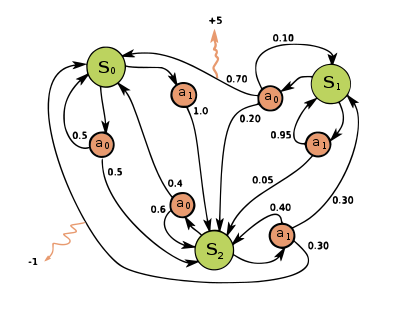
\includegraphics[height=6cm]{Markov_Decision_Process.svg.png}}
\end{frame}

\begin{frame}
  \frametitle{MDP Objective}
  \begin{itemize}
  \item The goal of the MDP is to find a good policy for a decision maker
  \item The policy $\pi(s)$ specifies the optimal action in each state
    and the resulting execution is a Markov chain
  \item Objective is to choose a policy $\pi$ that maximizes the cummulative reward, typically with a discount factor, i.e.
    \[ E\left[  \sum_t \gamma^t R_{a_t}(s_t, s+_{t+1}) \right] \]
  \item where $\gamma$ is a discount factor $0 \leq \gamma \leq 1$
    typically close to 1. A lower discount factor will encourage
    actions earlier
  \end{itemize}
\end{frame}

\begin{frame}
  \frametitle{Algorithms}
  \begin{itemize}
  \item The MDP can be solved using linear programming
    \begin{itemize}
    \item The optimal policy can be found using value function iteration.
      \begin{enumerate}
      \item Update Value: $V(s) = \sum_{s'} P_{\pi}(s,s') (R_{\pi}(s,s') + \gamma V(s'))$
      \item Policy update: $\pi(s) = \arg\max_a \left\{ \sum_{s'} P_{\pi}(s,s') (R_{\pi}(s,s') + \gamma V(s'))\right\}$
      \end{enumerate}
    \end{itemize}
  \item If the reward function is unknown this is an RL problem
    \begin{itemize}
    \item $Q(s,a) = \sum_{s'} P_{a}(s,s') (R_{a}(s,s') + \gamma V(s'))$
    \item Collecting $(s,a,s')$ triplets allow optimization and estimation of Q (so also as Q-learning)
    \end{itemize}
  \end{itemize}
\end{frame}


\begin{frame}
  \frametitle{Summary}
  \begin{itemize}
  \item Many types of time sequences can be described as a Markov chain or a Hidden Markov Model (HMM)
  \item The underlying theory is simple to understand
  \item You can describe the model as a graph / tree structure
  \item It is possible to capture the model with a transition matrix and an initial distirbution
  \item It is possible to learn / adapt the probabilities over time
  \item Widely used for temporal processes such as gestures, pose analysis, navigation, ...
  \item Numerous toolkits available for analysis and learning models.
  \end{itemize}
\end{frame}

\end{document}
